\section{Dijkstras algoritme} \label{kap:dijkstras}
I \autoref{defn:min.vej} definerede vi distancen af den korteste vej i en vægtet graf. For at finde den korteste vej vil vi anvende \emph{Dijkstras algoritme}. Dijkstras algoritme kan bruges til at finde den korteste vej i en simpel, vægtet graf, hvori vægtene for alle kanter i grafen skal være ikke-negative. Algoritmen fungerer således, at den finder den korteste vej fra en startknude, $v_{1}$, til en endeknude, $v_{m}$, ved først at finde naboknuderne til $v_{1}$ og undersøge hvilken af disse, der har den mindste distanceværdi og altså er tættest på startknuden. Derefter tager den udgangspunkt i den naboknude, hvortil distanceværdien er mindst og fortsætter ad dennes vej, så længe denne vej har en mindre distanceværdi end en alternativ vej. Fremgangsmåden vil her illustreres ved hjælp af et eksempel, som tager udgangspunkt i \autoref{kap:grafteori}.

\begin{exmp} \label{exmp.dijkstae}

I \autoref{fig.dijkstraexmp} vil vi finde den korteste vej fra $v_{1}$ til $v_{6}$. Dijkstras algoritme vil gøre dette ved at finde den korteste vej fra startknuden, $v_{1}$, til hver knude, indtil den når endeknuden, $v_{6}$. Først vil den se, at startknuden har naboknuderne $v_{2}$ og $v_{3}$. Der er altså to veje fra startknuden, $P_1=(v_{1},v_{2})$  og $P_2=(v_{1},v_{3})$, hvor $\dist(P_1)=5$ og $\dist(P_2)=3$. Dermed er $v_{3}$ den knude, der er tættest på startknuden. Herefter er der igen to veje, $P_1$ og $P_3=(v_{1},v_{3},v_{5})$, hvor $\dist(P_3)=7$. $P_1$ vælges, da denne har den mindste distance, og $v_{2}$ er dermed knuden, som er næsttættest på startknuden. Nu er der tre forskellige veje, $P_3=(v_{1},v_{3}, v_{5})$, 
$P_4=(v_{1},v_{2}, v_{4})$ og $P_5=(v_{1},v_{2}, v_{5})$, hvor $\dist(P_4)=9$ og $\dist(P_5)=9$. $P_3$ vælges, og det er nu noteret, at $\alpha(v_{1},v_5)=7$. Der er nu igen kun to mulige veje at vælge imellem, $P_4$ og $P_6=(v_{1},v_{3}, v_{5}, v_{6})$, hvor $\dist(P_6)=8$. $P_5$ er ikke længere en mulig vej, da vi allerede har fundet den korteste vej fra $v_{1}$ til $v_{5}$. $P_6$ har den mindste distance, og derfor vælger vi denne, og vi ved nu, at den korteste vej fra $v_{1}$ til $v_{6}$ er $P_6=(v_{1},v_{3}, v_{5}, v_{6})$, altså $\alpha(v_1,v_6)=8$.
\begin{figure}[H]
\centering
	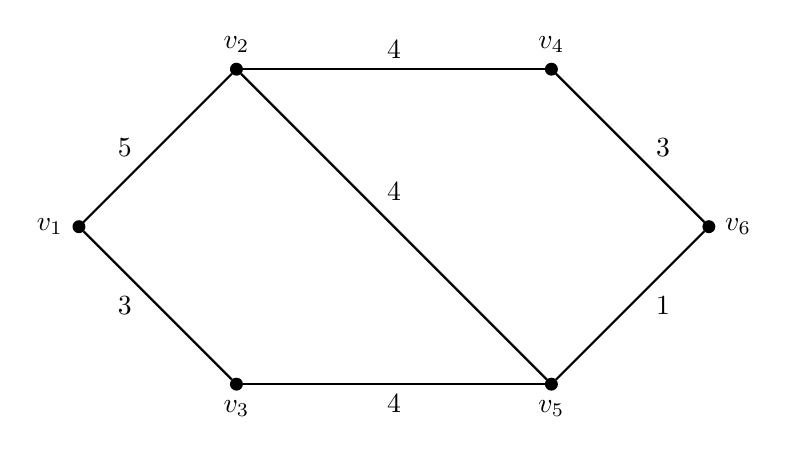
\begin{tikzpicture}

      \tikzset{enclosed/.style={draw, circle, inner sep=0pt, minimum size=.15cm, fill=black}}
%% Vertices
      	\node[enclosed, label={left: $v_1$}] (v1) at (0,2) {};
      	\node[enclosed, label={above: $v_2$}] (v2) at (2,4) {};
    	\node[enclosed, label={below: $v_3$}] (v3) at (2,0) {};
  	    \node[enclosed, label={above: $v_4$}] (v4) at (6,4) {};
     	\node[enclosed, label={below: $v_5$}] (v5) at (6,0) {};
     	\node[enclosed, label={right: $v_6$}] (v6) at (8,2) {};
%Edges
		\path [-, > = latex, thick] (v1) edge node[midway, left=2mm] {$ 5 $} (v2);
		\path [-, > = latex, thick] (v1) edge node[midway, left=2mm] {$ 3 $} (v3);
		\path [-, > = latex, thick] (v2) edge node[midway, above] {$ 4 $} (v4);
		\path [-, > = latex, thick] (v2) edge node[midway, above=2mm] {$ 4 $} (v5);
		\path [-, > = latex, thick] (v3) edge node[midway, below] {$ 4 $} (v5);
		\path [-, > = latex, thick] (v4) edge node[midway, right=2mm] {$ 3 $} (v6);
		\path [-, > = latex, thick] (v5) edge node[midway, right=2mm] {$ 1 $} (v6);

	\end{tikzpicture}
	\caption{Simpel, vægtet graf.}
	\label{fig.dijkstraexmp}
\end{figure}
\end{exmp}

Ovenstående eksempel er simpelt og kan hurtigt løses ved fx brute force men i større og mere komplicerede grafer er Dijkstras algoritme meget mere effektiv. For at skabe yderligere overblik over hvordan Dijkstras algoritme fungerer, vil vi her gå i dybden med dennes mere teoretiske del.
\begin{algorithm}[H]
\caption{Dijkstras algoritme}
\begin{algorithmic}[1]

\Procedure{dijkstra($G$: vægtet, sammenhængende, simpel graf med kun ikke-negative vægte)}{}
    \State \{$G$ {har knuderne $a = v_{1}, v_{2}, \dotsc, v_{m} = z$ og vægtene til kanterne $w(v_{i}, v_{j})$, hvor $w(v_{i}, v_{j}) = \infty$ hvis $v_{i}$ og $v_{j}$ ikke er naboer \}}
	\For {$i := 2$ \textbf{to} $m$}
		\State $L(v_{i}) := \infty$
	\EndFor
	\State $L(a) := 0$	
	\State $S := \emptyset$
	\State {\{distancen til hver knude initialiseres, så $a = 0$, og distancen til alle andre knuder er $\infty$, derudover er $S$ defineret som en tom mængde\}}
    \While{$z \notin S$}
        \State {$u :=$ en knude som ikke er i $S$ med $L(u)$ som minimum}
        \State $S := S \cup \{u\}$
        \For {alle $v \notin S$}
        	\If {$L(u) + w(u,v) < L(v)$} {$L(v) := L(u) + w(u,v)$}
        	\State \{dette tilføjer knuder til $S$ med minimal 			distance og opdaterer distancerne til
        	\State knuderne, som ikke er i $S$\}
        	\EndIf
    	\EndFor
    \EndWhile
    \State {\textbf{return} $L(z)$ \{$L(z) = \alpha(a,z)$\}} 
\EndProcedure

\end{algorithmic}
\label{alg:dijkstra}
\end{algorithm}
Det første, der sker, er, at distancen til startknuden noteres som $0$, og til resten af knuderne som $\infty$. Derudover oprettes en mængde, $S$, for hvilken det gælder, at $S = \emptyset$ når $k = 0$, hvor $k$ er antallet af iterationer gennemført i algoritmen, altså antallet af gange $S$ opdateres. Distancen af den korteste vej algoritmen finder fra startknuden til en given knude, noterer vi her ved $L$. $L_{0}(v_1)=0$ betyder altså, at vi har nul iterationer og dermed kun kender startknuden med distancen $0$. . Ved første iteration undersøges startknudens naboknuder, og man bestemmer, som i eksemplet ovenfor, hvilken distance er mindst. Dermed er startknudens nærmeste knude fundet, og denne tilføjes nu til $S$. For hver iteration tilføjes et nyt element til mængden, og denne proces fortsætter, til algoritmen har fundet den korteste vej fra startknuden til endeknuden. Mængden, $S$, indeholder til sidst distancerne for den korteste vej fra startknuden til alle knuder i grafen. 

Ved brug af ovenstående metode kan vi illustrere løsningen til korteste vej-problemet fra \autoref{fig.dijkstraexmp} i en tabel.

\begin{table}[H]
\centering
\begin{tabular}{|c|c|c|c|c|c|c|}
\hline
$v$ & $v_1$ & $v_2$ & $v_3$ & $v_4$ & $v_5$ & $v_6$ \\ \hline
  & $\boldsymbol{0}$ &  $\infty$ & $\infty$  & $\infty$  &  $\infty$  &  $\infty$  \\  
 $v_1$ &  & $5_{v_1}$ & $\boldsymbol{3_{v_1}}$ & $\infty$ & $\infty$ & $\infty$ \\  
 $v_3$ &  & $\boldsymbol{5_{v_1}}$ &  & $\infty$ & $7_{v_3}$ & $\infty$ \\  
 $v_2$ &  &  &  & $9_{v_2}$ & $\boldsymbol{7_{v_3}}$ & $\infty$ \\
 $v_5$ &  &  &  & $9_{v_2}$ &  & $\boldsymbol{8_{v_5}}$   \\ \hline
\end{tabular}
\caption{Tabellarisk løsning til korteste vej i \autoref{fig.dijkstraexmp}.}
\label{tab:dijkstraexmp}
\end{table}

\begin{thm}[Dijkstras algoritme] \label{thm:dijkstra}
Dijkstras algoritme finder distancen af den korteste vej mellem to knuder, $a$ og $z$, i en vægtet, sammenhængende og simpel graf, sådan at $L(z)=\alpha(a,z)$. 
\end{thm}

\begin{proof}
Sætning \ref{thm:dijkstra} kan bevises ved induktion. Ved et induktionsbevis etablerer vi først et basisskridt, og dernæst opstiller vi en induktionshypotese. Basisskridtet består blot i, at vi undersøger distancen fra startknuden til startknuden, som selvfølgelig er 0, hvilket algoritmen også noterer. Vi har dermed $L(a)=0= \alpha(a,a)$, hvilket er sandt.
Vi opstiller nu vores induktionshypotese, hvor vi antager, at Sætning \ref{thm:dijkstra} er sand for $k$ iterationer. Det gælder altså, at

\begin{equation}
L(u) = \alpha(a,u), \forall u \in S_k. 
\end{equation} %usikker på denne
Vi sætter nu $v$ til at være den knude, der tilføjes til $S$ ved $S_{k+1}$. Vi vil nu vise, at det ligesom ved alle tidligere knuder i $S$ også gælder for $v$ at $L(v)=\alpha(a,v)$. Dette kan bevises ved modstrid. Vi starter med at antage, at der findes en kortere vej fra $a$ til $v$ end $L(v)$. Vi kalder denne nye vej $P_1$. For denne må det gælde, at

\begin{equation}
\dist(P_1)<L(v).
\end{equation} %Det er her det handler om, () eller {}
$P_1$ starter i $S_k$ og forlader på et tidspunkt denne mængde for at komme til $v$, som ikke er i $S_k$. Vi lader $\{x,y\}$ være den første kant på vejen $P_1$, der forlader $S_k$. $P_x$ betegnes som delen af vejen $P_1$, som går fra $a$ til $x$. Så ved vi, at

\begin{equation}
\dist(P_x)+w(x,y) \leq \dist(P_1).
\end{equation}
Eftersom $x$ er i $S_k$, ved vi som følge af induktionshypotesen, at den korteste vej fra $a$ til $x$ er $L(x)$. Dermed ved vi, at $L(x) \leq \dist(P_x)$ og

\begin{equation}
L(x) + w(x,y) \leq \dist(P_1).
\end{equation}
$y$ er nabo til $x$, hvilket betyder, at

\begin{equation}
L(y) \leq L(x) + w(x,y).
\end{equation}
Eftersom hverken $v$ eller $y$ er i $S_k$, og algoritmen oprindeligt valgte $v$ i den $(k+1)$'te iteration, må $v$ have den mindste distance af de to således, at

\begin{equation}
L(v) \leq L(y).
\end{equation}
Dette resulterer dog i, at vi påstår, at $L(v) < L(v)$. Dette kan ikke lade sig gøre, og vi konkluderer derfor, at der ikke findes en tilfældig kortere vej, $P_1$. $L(v)=\alpha(a,v)$ må altså være sandt, og Dijkstras algoritme finder den korteste vej.
\end{proof}
